\documentclass[12pt]{article}
\usepackage{graphicx}
\usepackage{setspace}
\usepackage{fancyhdr}
\usepackage{amssymb}
\usepackage{xcolor}
\usepackage{amsmath}
\usepackage{svg}
\usepackage[colorlinks=true, urlcolor=blue]{hyperref}
\usepackage{graphicx}
\usepackage{makecell}
\usepackage{fontawesome5}
\usepackage[a4paper, margin=1in]{geometry}
\pagestyle{fancy}
\lhead{Spherical Wavelet Implementation}
\rhead{Aliakbar Zarkoob}

\begin{document}
	
	\begin{titlepage}
		\begin{center}
			
			
\includegraphics[height=4cm]{University_of_Tehran_Transparent_BW_logo.png} \hfill
			
\includegraphics[height=4cm]{Fanni_Alt_BW_Logo.png}
			
			\vspace{1cm}
			
			\Large \textbf{School of Surveying and Geospatial Engineering}\\
			\large {Department of Geodesy and Hydrography}
			
			\vspace{3cm}
			
			\huge \textbf{Spherical Wavelet Implementation}\\
			\large \href{https://github.com/XIVAliakbarZarkoob/Spherical-Wavelets}{\faGithub}
			
			\vspace{3cm}
			
			\Large \textbf{Author:}\\
			\Large Aliakbar Zarkoob
			
			\vspace{2cm}
			
			\Large \textbf{Professor:}\\
			Dr. AbdolReza Safari
			
			\vfill
			
			\large {Winter 2025}
			
		\end{center}
	\end{titlepage}
	
	
	\section{Introduction}
	
	In recent years, the application of spherical wavelet transforms has emerged as a powerful tool for analyzing geophysical data, particularly in the context of gravity potential fields. Spherical wavelets offer a multi-resolution framework that allows for the effective decomposition of complex data structures. Unlike traditional techniques, spherical wavelets preserve the inherent characteristics of the data while providing localized frequency information. This capability is particularly advantageous in geophysical studies, where the spatial and temporal variations of potential fields can be intricate. 
	
	This report focuses on the implementation of spherical wavelets using the Shannon scale function, specifically applied to gravity potential data derived from the WHU-SWPU-GOGR2022S model. The data is organized in a global grid with a uniform step size of 1 degree. The Driscoll-Healy method, a numerical approach for spherical harmonics, serves as a foundation for this implementation.
	
	\section{Implementation Steps}
	
	As mentioned before, the data used in this project is gravity potential from WHU-SWPU-GOGR2022S model. This data was acquired from ICGEM \footnote{International Center for Global Earth Models: \url{https://icgem.gfz-potsdam.de}}, and it's shown in the figure \ref{fig:MainData}.
	
	\begin{figure}[h!]
		\centering
		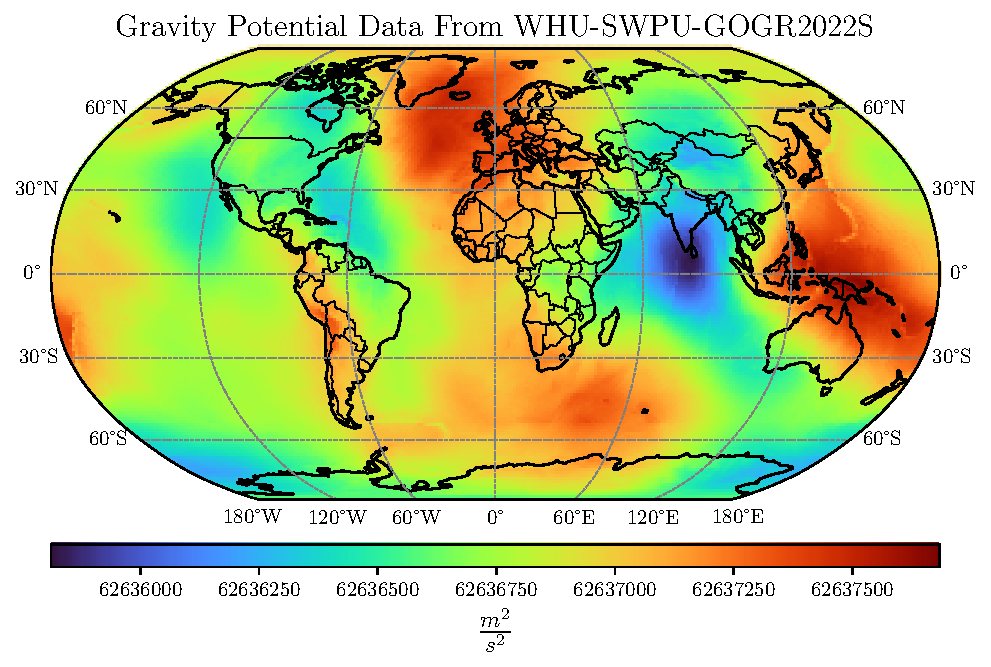
\includegraphics[height=7cm]{../Outputs/Plots/MainData.pdf}
		\caption{Gravity potential data from WHU-SWPU-GOGR2022S model.}
		\label{fig:MainData}
	\end{figure}
	
	The scale-spaces and wavelet-spaces are defined based on the multi-resolution analysis (MRA) as shown in equation \ref{eq:MRA}.
	
	\begin{equation}
		\begin{cases} 
			V_J = \left\{\Phi_J^{(2)}*F|F\in\mathbb{L}^2(\Omega)\right\} \\
			W_J = \left\{\tilde{\Psi}_J*\Psi_J*F|F\in\mathbb{L}^2(\Omega)\right\}
		\end{cases}
		\label{eq:MRA}
	\end{equation}
	
	The detailed and Smooth parts of input function are defined as equation \ref{eq:SD}.
	
	\begin{equation}
		\begin{cases} 
			P_J(F) = \Phi_J^{(2)}*F \in V_J \\
			R_J(F) = \tilde{\Psi}_J*\Psi_J*F \in W_J
		\end{cases}
		\label{eq:SD}
	\end{equation}
	
	As mentioned before, Shannon scale function is used in this project. This scale function and the corresponding wavelet function is shown in equation \ref{eq:Shannon}. Thus, the input function can be written as equation \ref{eq:WaveletSeries}.
	
	\begin{equation}
		\begin{cases} 
			\Phi_J(\xi,\eta) = \displaystyle \sum_{n=0}^{2^J-1} \frac{2n+1}{4\pi}P_n(\xi.\eta) \\
			\tilde{\Psi}_J(\xi,\eta)=\Psi_J(\xi,\eta) = \displaystyle \sum_{n=0}^{2^{J+1}-1} P_n(\xi.\eta)
		\end{cases}
		\label{eq:Shannon}
	\end{equation} 
	
	\begin{equation}
		\begin{split}
			&F = \Phi_0^{(2)}*F + \displaystyle \sum_{j=0}^{J} \int_{\Omega}WT(F,j)\Psi_J(\eta)dw(\eta) \\
			&WT(F,j) = \Psi_j * F = \int_{\Omega}\Psi_j(\xi,\eta)F(\eta)dw(\eta)
			\label{eq:WaveletSeries} 
		\end{split}
	\end{equation}
	
	Based on Driscoll-Healy method:
	
	\begin{equation}
		R_J(F) = \displaystyle \sum_{i=0}^{2^{J+2}-1} \sum_{j=0}^{2^{J+2}-1} w_iWT_F(J,\eta_{ij})\Psi_J(\xi.\eta_{ij}^T)
	\end{equation}
	
	\begin{equation}
		WT_F(J,\eta_{ij}) = \displaystyle \sum_{i=0}^{2^{J+1}-1} \sum_{j=0}^{2^{J+1}-1} a_{ij}^T \Psi_J(\xi.\eta_{ij}^T)
	\end{equation}
	
	\begin{equation}
		a_{ij}^T = w_jF(\eta_{ij}^T)
	\end{equation}
	
	\begin{equation}
		w_j = \frac{4}{m+1} \sin\left(\frac{j\pi}{m+1}\right) \displaystyle \sum_{s=0}^{\frac{m+1}{2}-1} \frac{1}{2s+1} \sin\left((2s+1)\frac{j\pi}{m+1}\right)
	\end{equation}
	\clearpage
	
	\section{Results}
	
	Smooth and detail parts of the given gravity potential function are shown in figures \ref{fig:Results1} to \ref{fig:Results8} for scales of 1 to 8.
	\begin{figure}[h!]
		\centering
		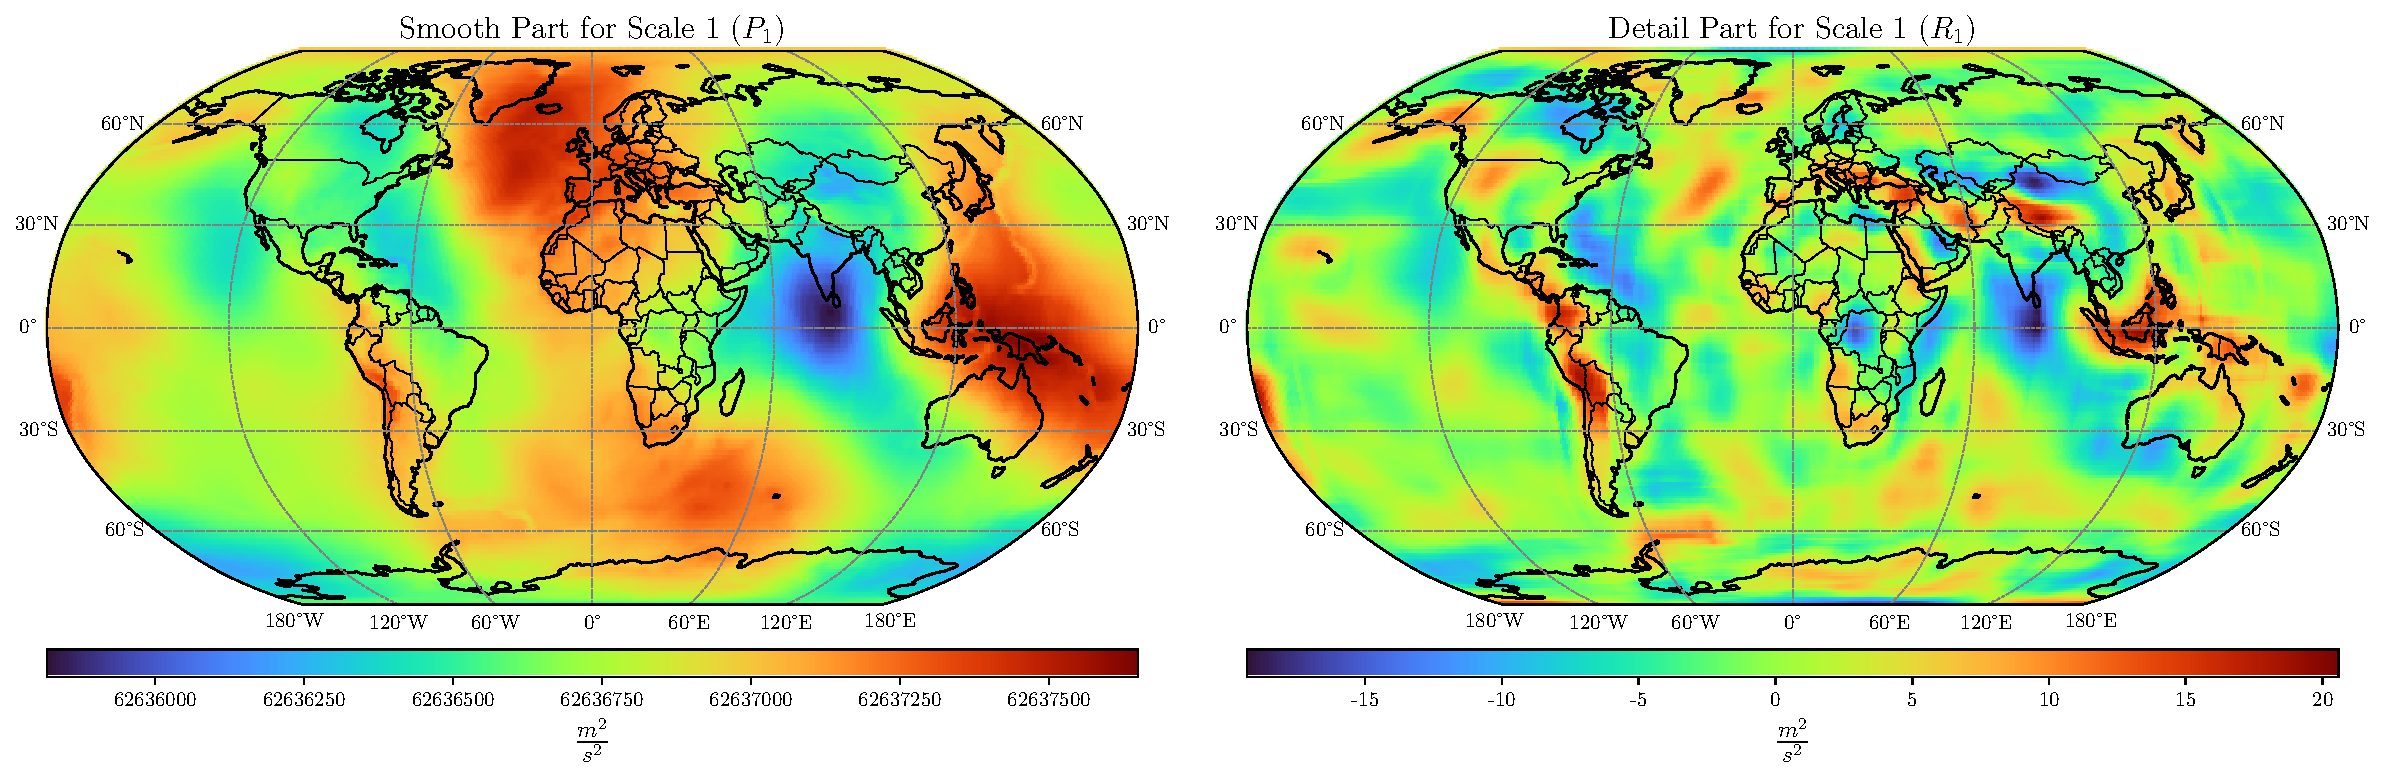
\includegraphics[width=16cm]{../Outputs/Plots/Outputs_Scale1.pdf}
		\caption{Smooth and detail part of scale 1.}
		\label{fig:Results1}
	\end{figure}
	
	\begin{figure}[h!]
		\centering
		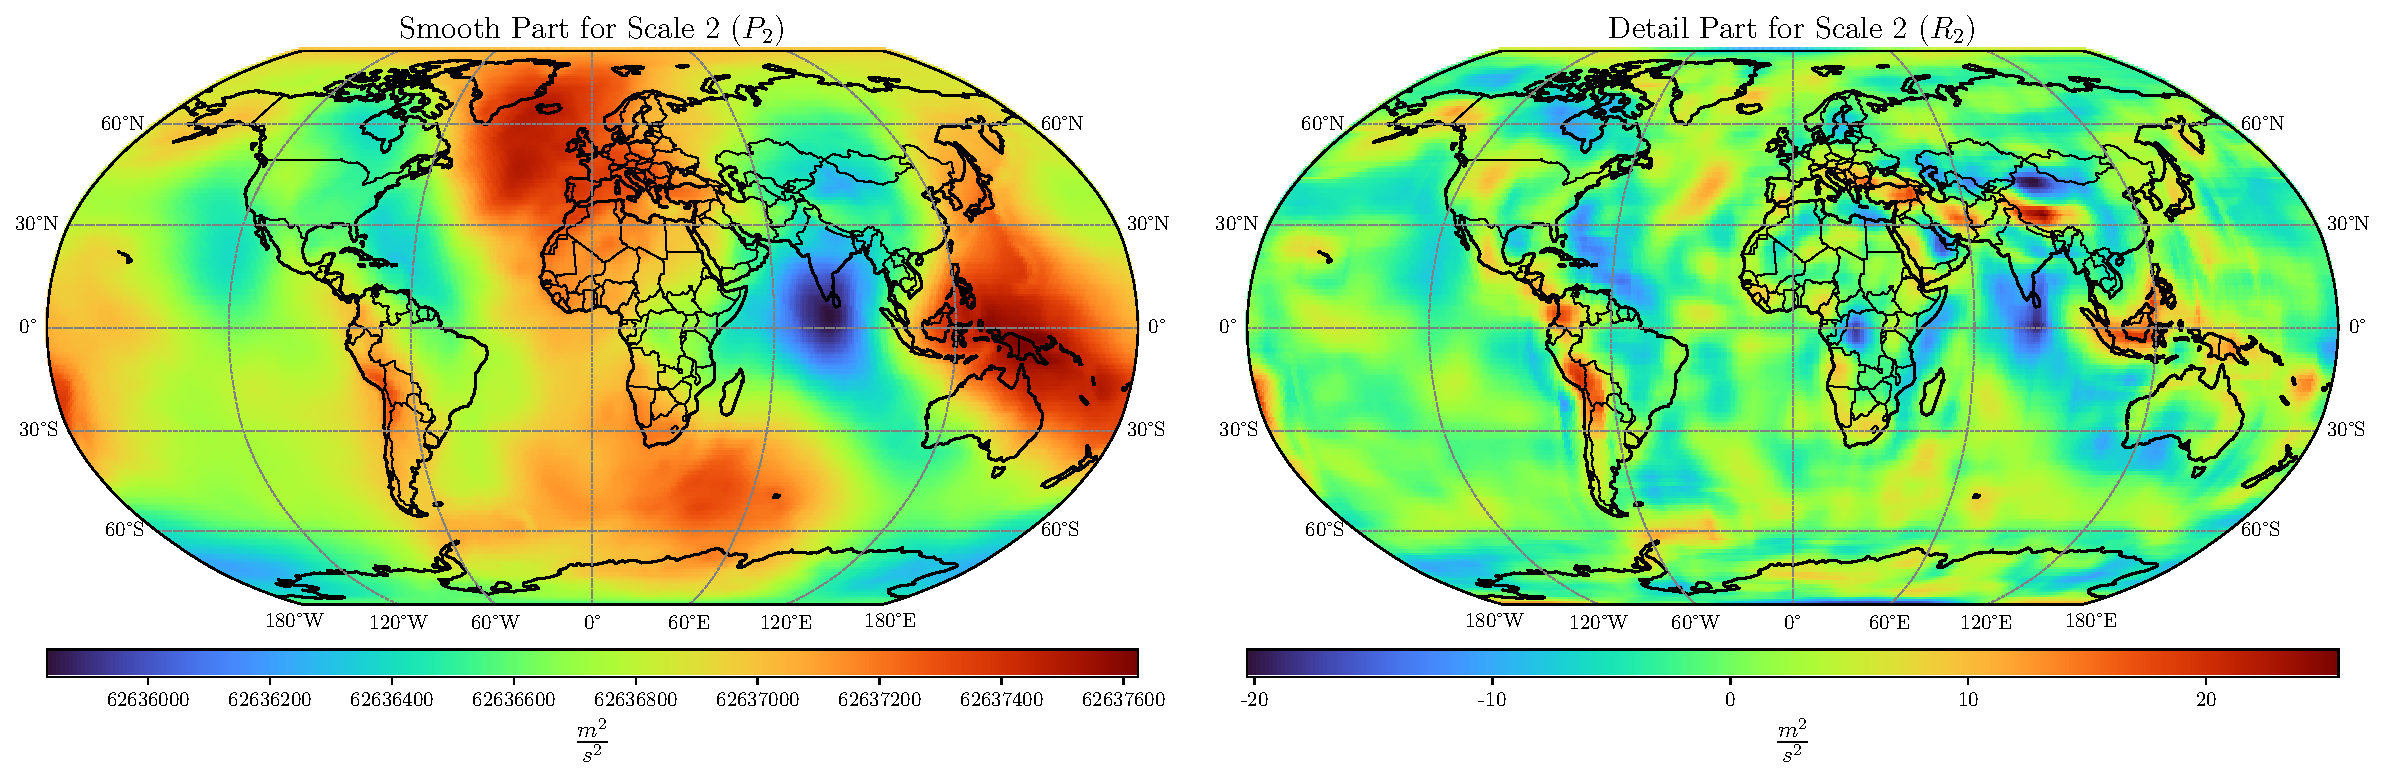
\includegraphics[width=16cm]{../Outputs/Plots/Outputs_Scale2.pdf}
		\caption{Smooth and detail part of scale 2.}
		\label{fig:Results2}
	\end{figure}
	
	\begin{figure}[h!]
		\centering
		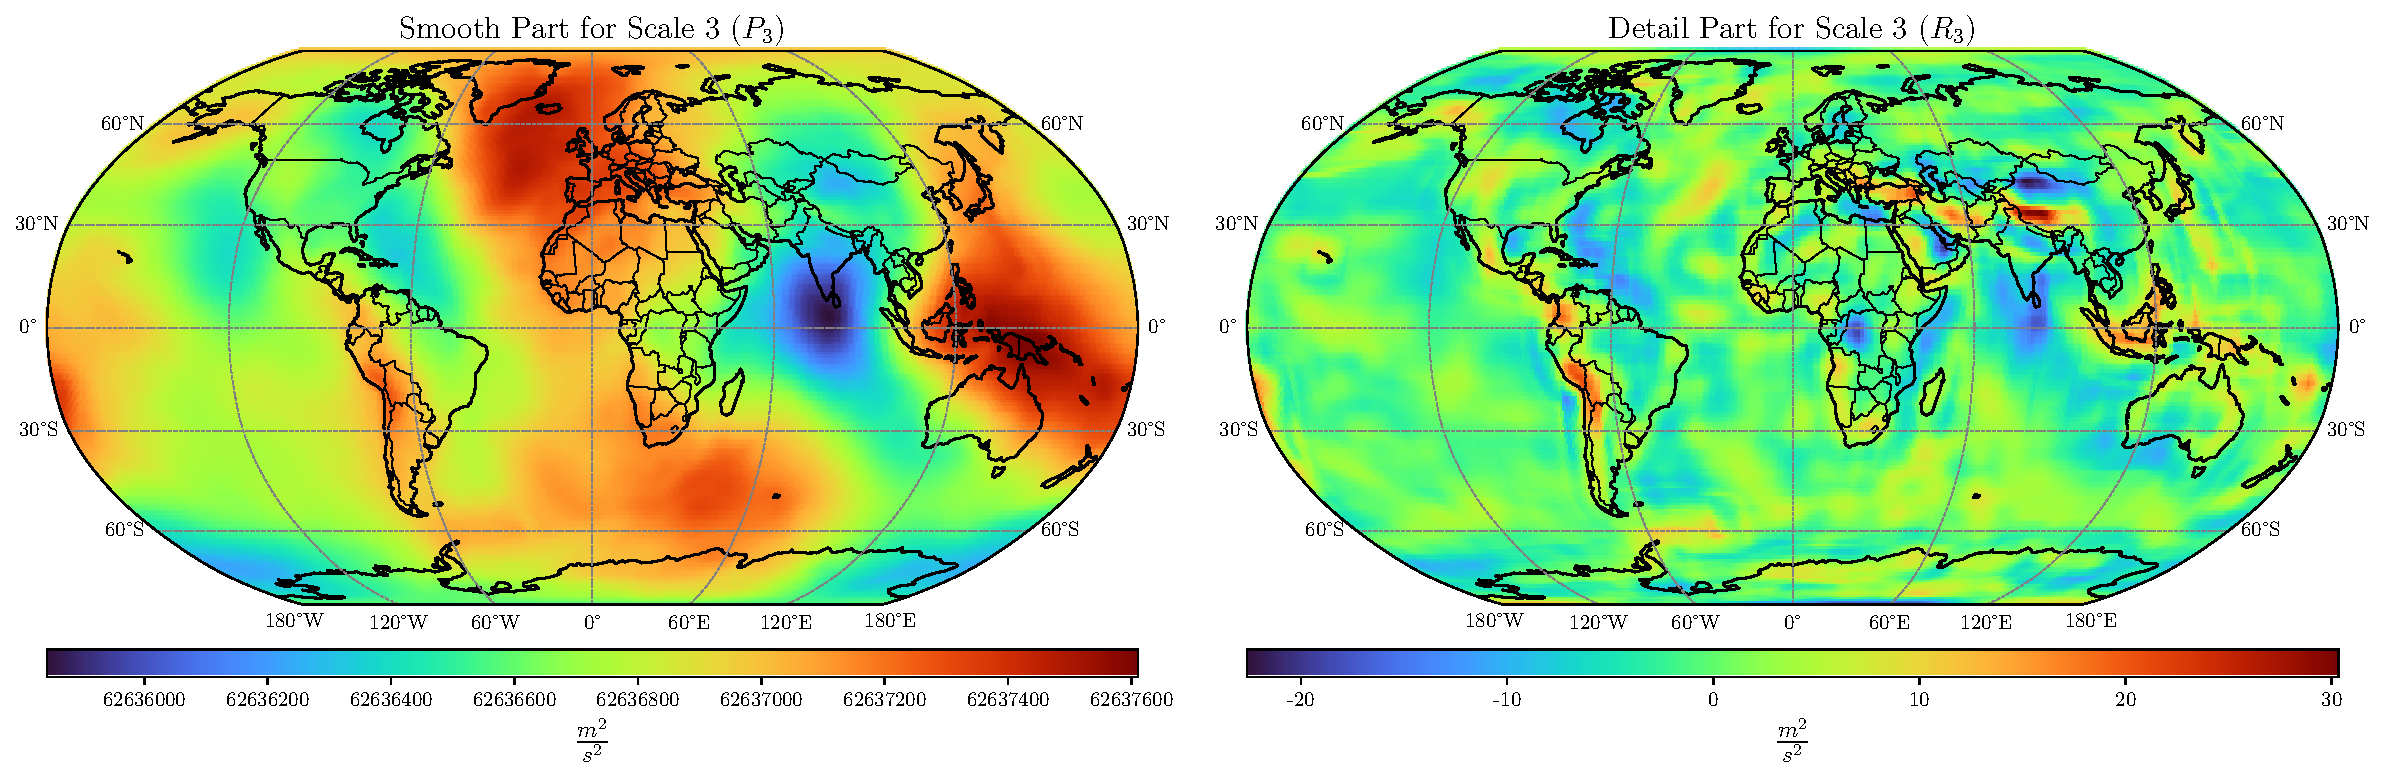
\includegraphics[width=16cm]{../Outputs/Plots/Outputs_Scale3.pdf}
		\caption{Smooth and detail part of scale 3.}
		\label{fig:Results3}
	\end{figure}
	
	\begin{figure}[h!]
		\centering
		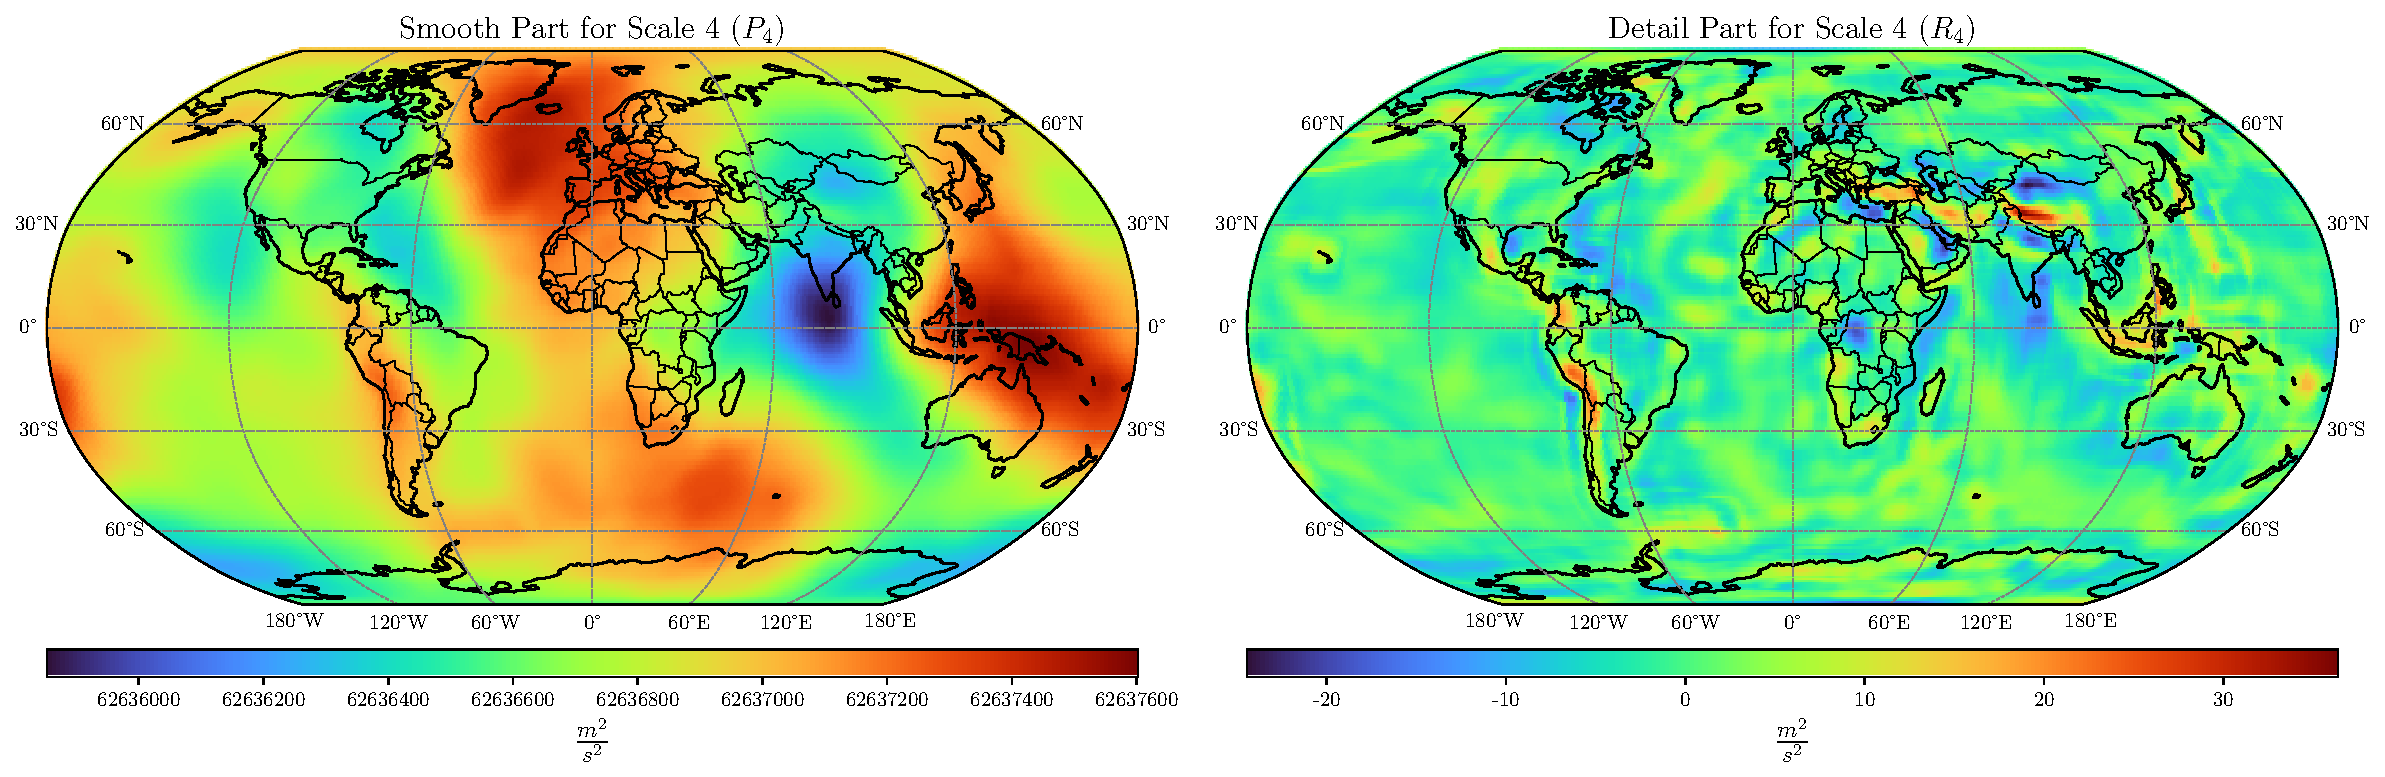
\includegraphics[width=16cm]{../Outputs/Plots/Outputs_Scale4.pdf}
		\caption{Smooth and detail part of scale 4.}
		\label{fig:Results4}
	\end{figure}
	
	\begin{figure}[h!]
		\centering
		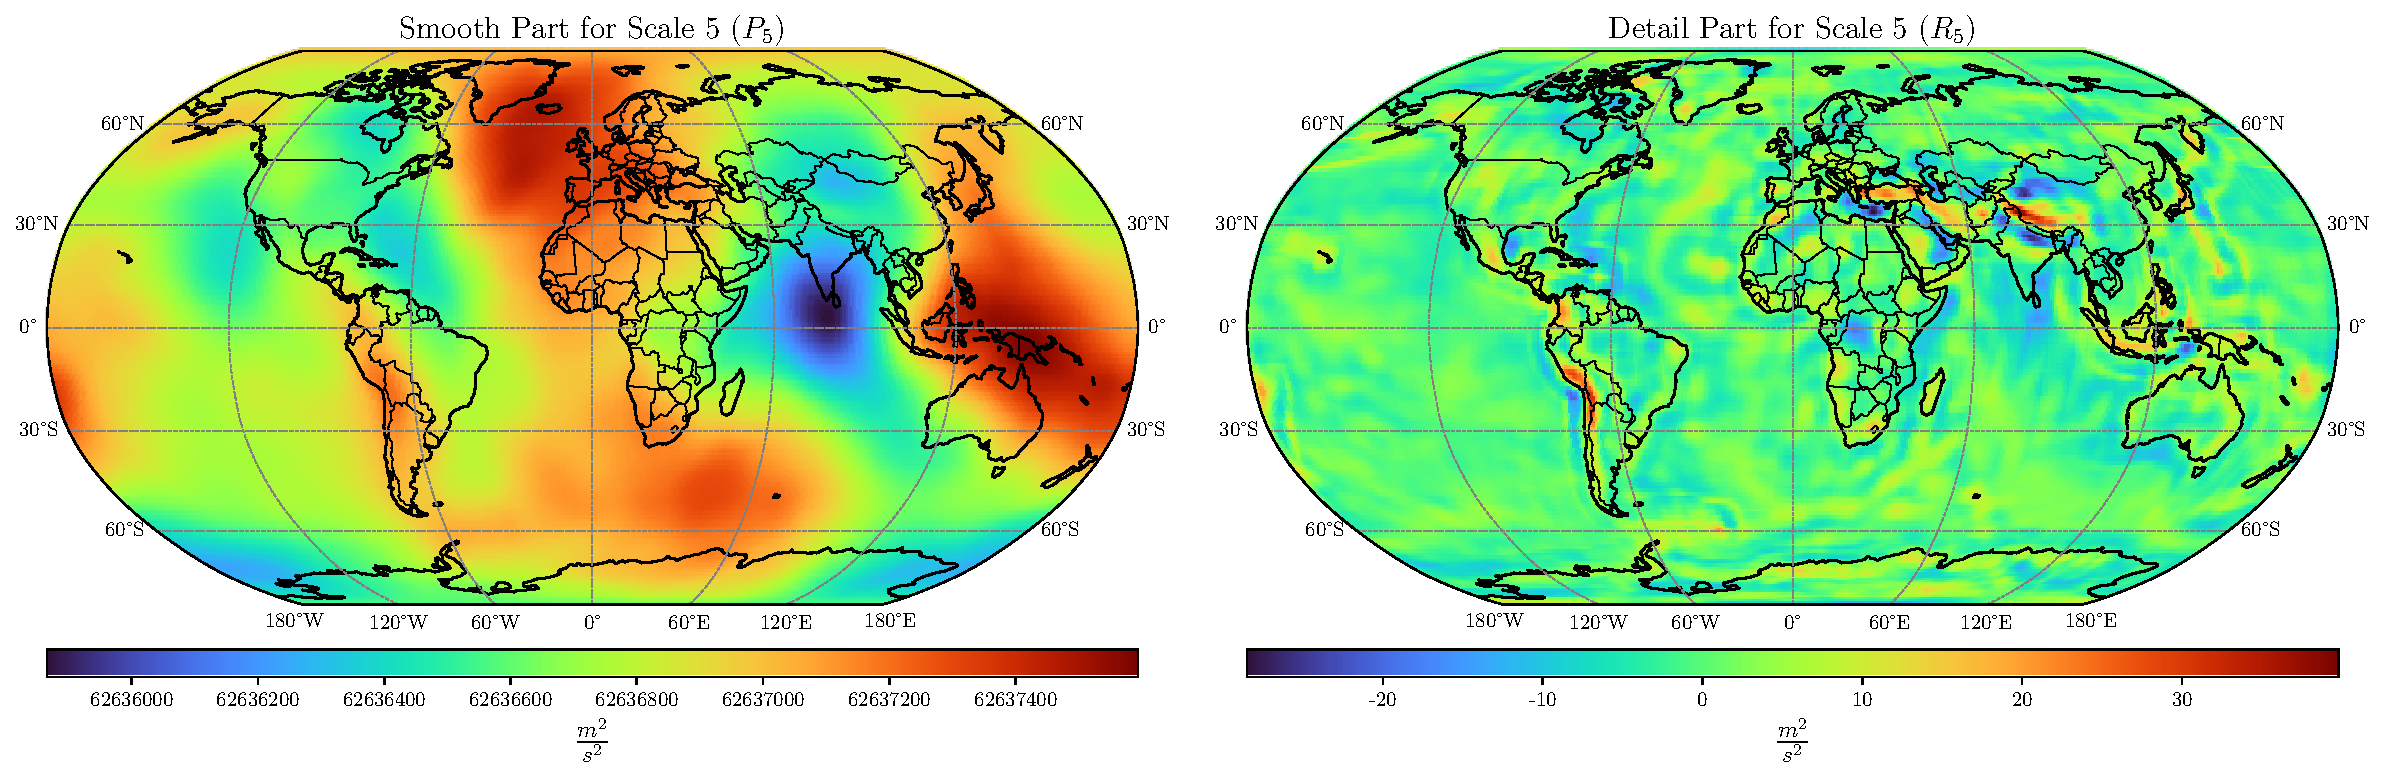
\includegraphics[width=16cm]{../Outputs/Plots/Outputs_Scale5.pdf}
		\caption{Smooth and detail part of scale 5.}
		\label{fig:Results5}
	\end{figure}
	
		\begin{figure}[h!]
		\centering
		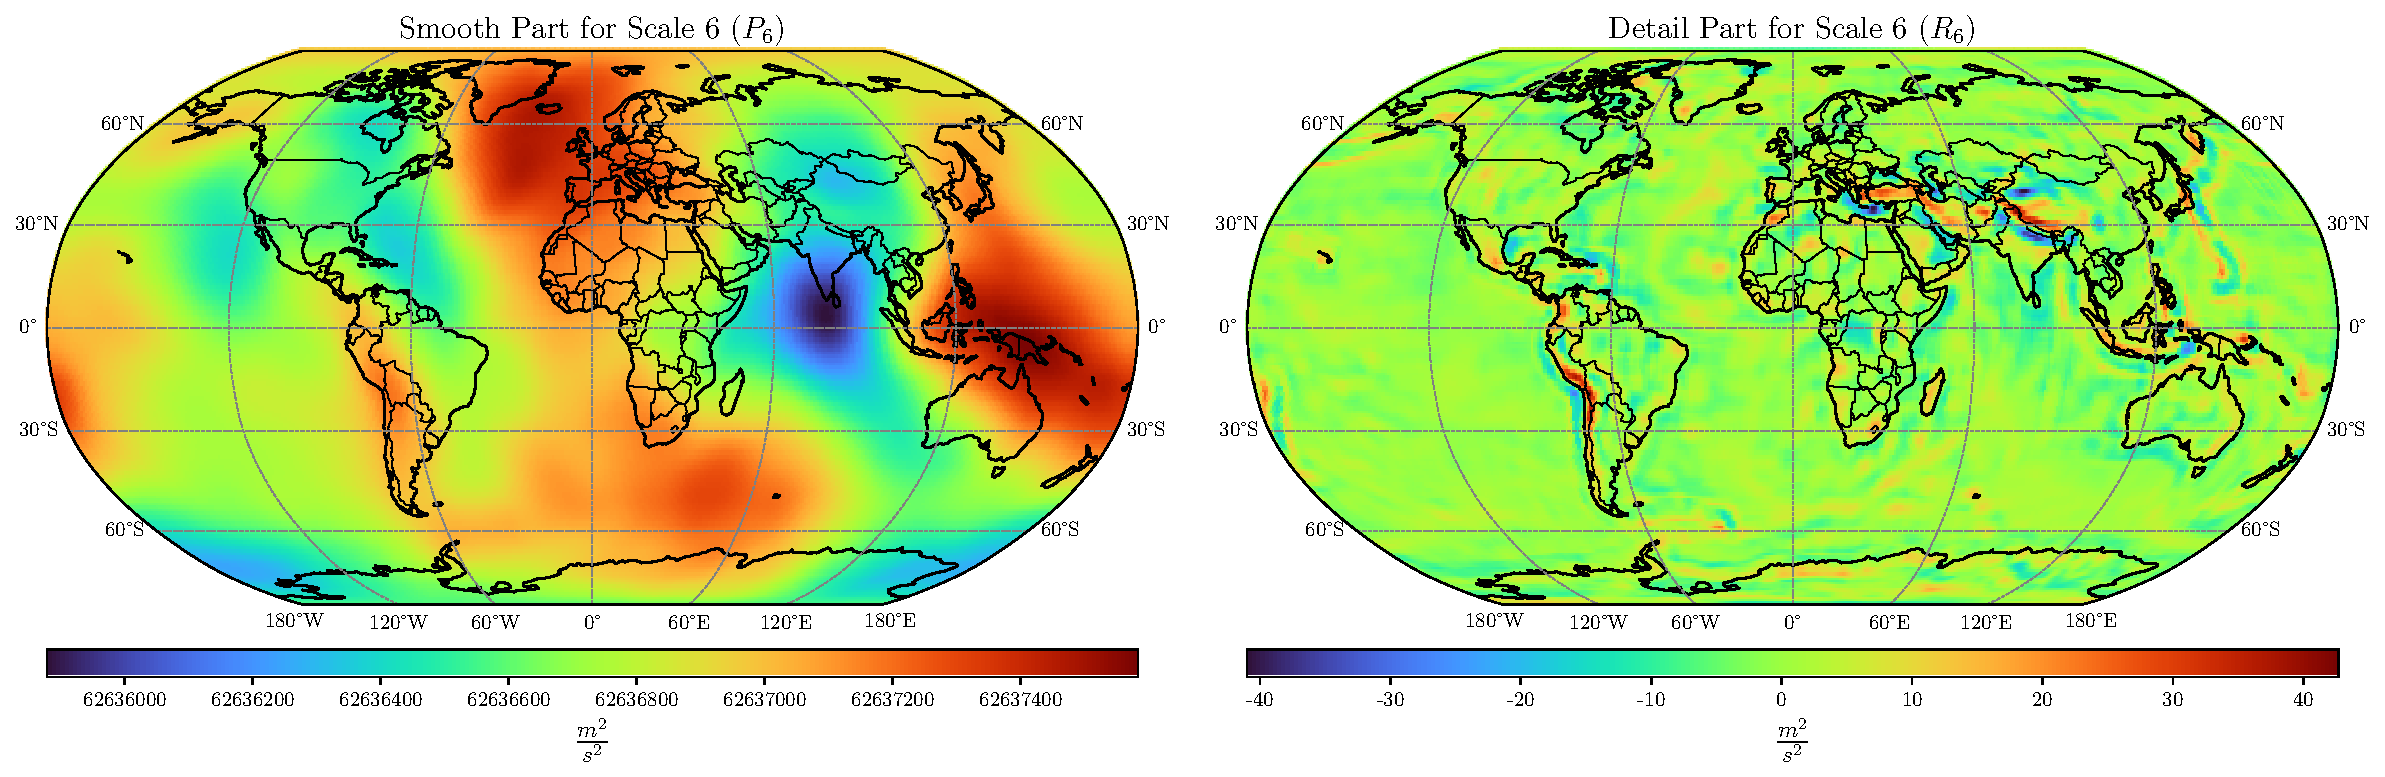
\includegraphics[width=16cm]{../Outputs/Plots/Outputs_Scale6.pdf}
		\caption{Smooth and detail part of scale 6.}
		\label{fig:Results6}
	\end{figure}
	
	\clearpage
	
	\begin{figure}[h!]
		\centering
		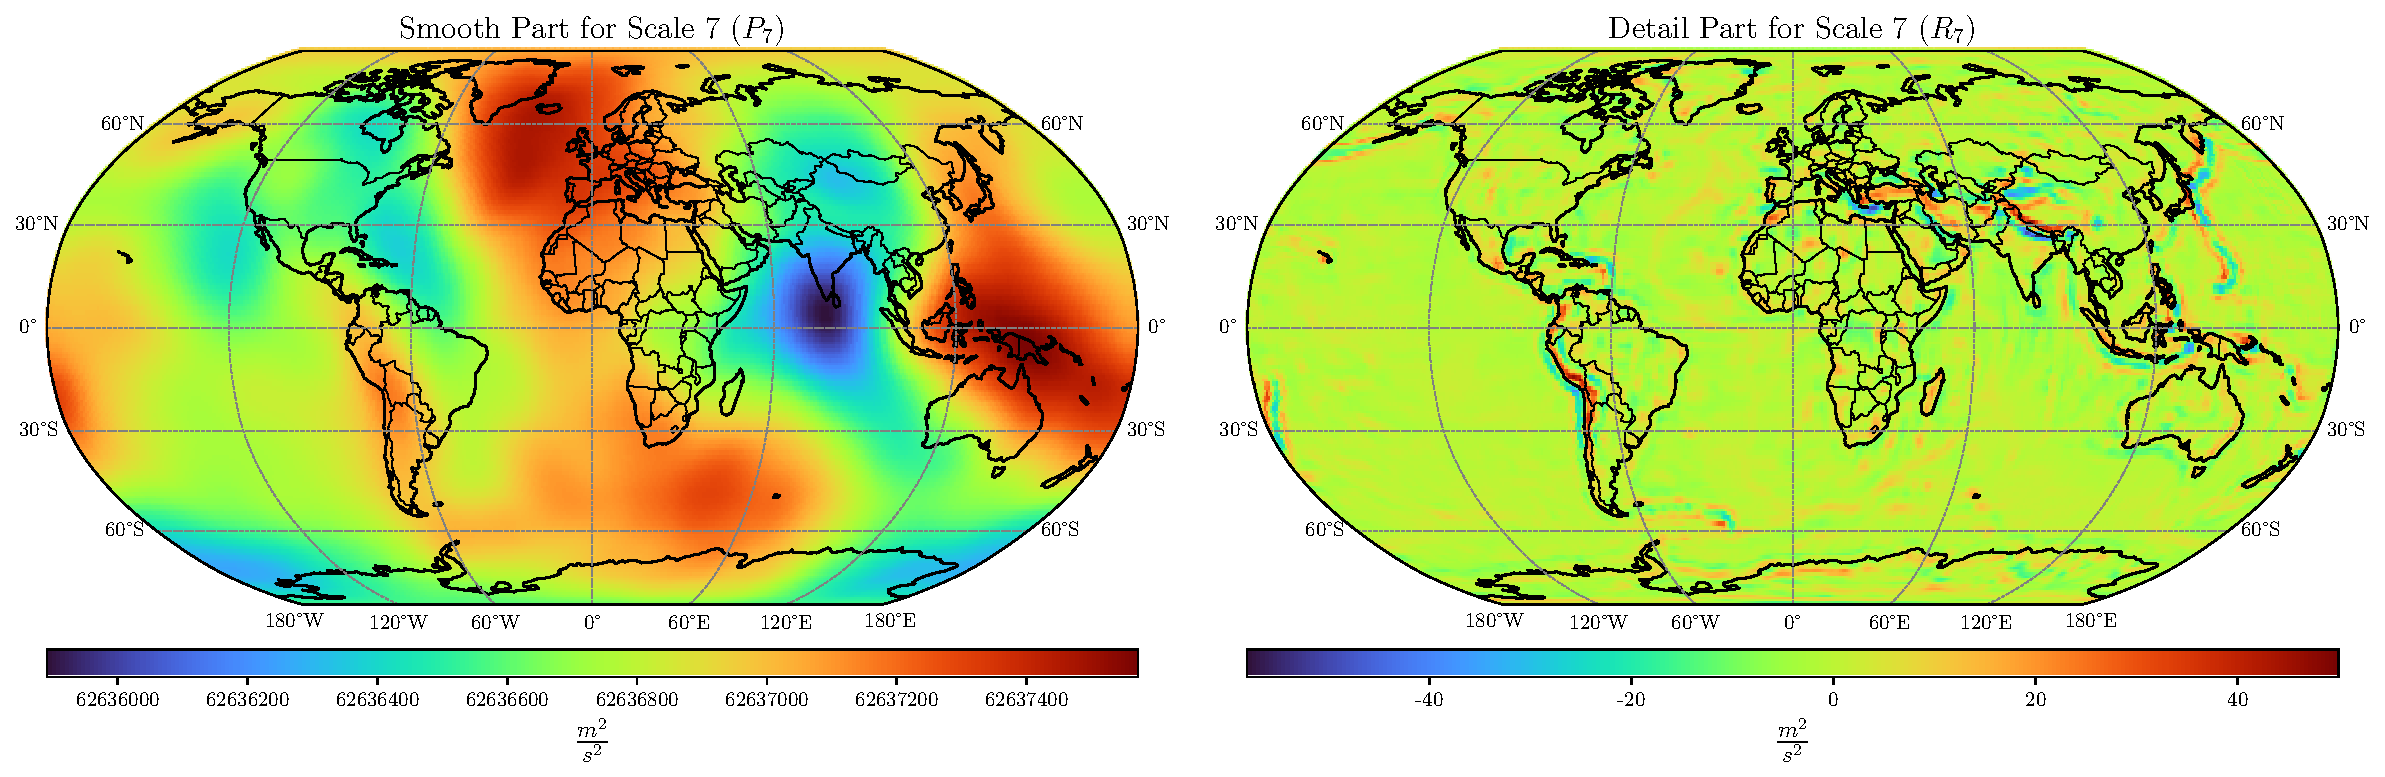
\includegraphics[width=16cm]{../Outputs/Plots/Outputs_Scale7.pdf}
		\caption{Smooth and detail part of scale 7.}
		\label{fig:Results7}
	\end{figure}
	
	\begin{figure}[h!]
		\centering
		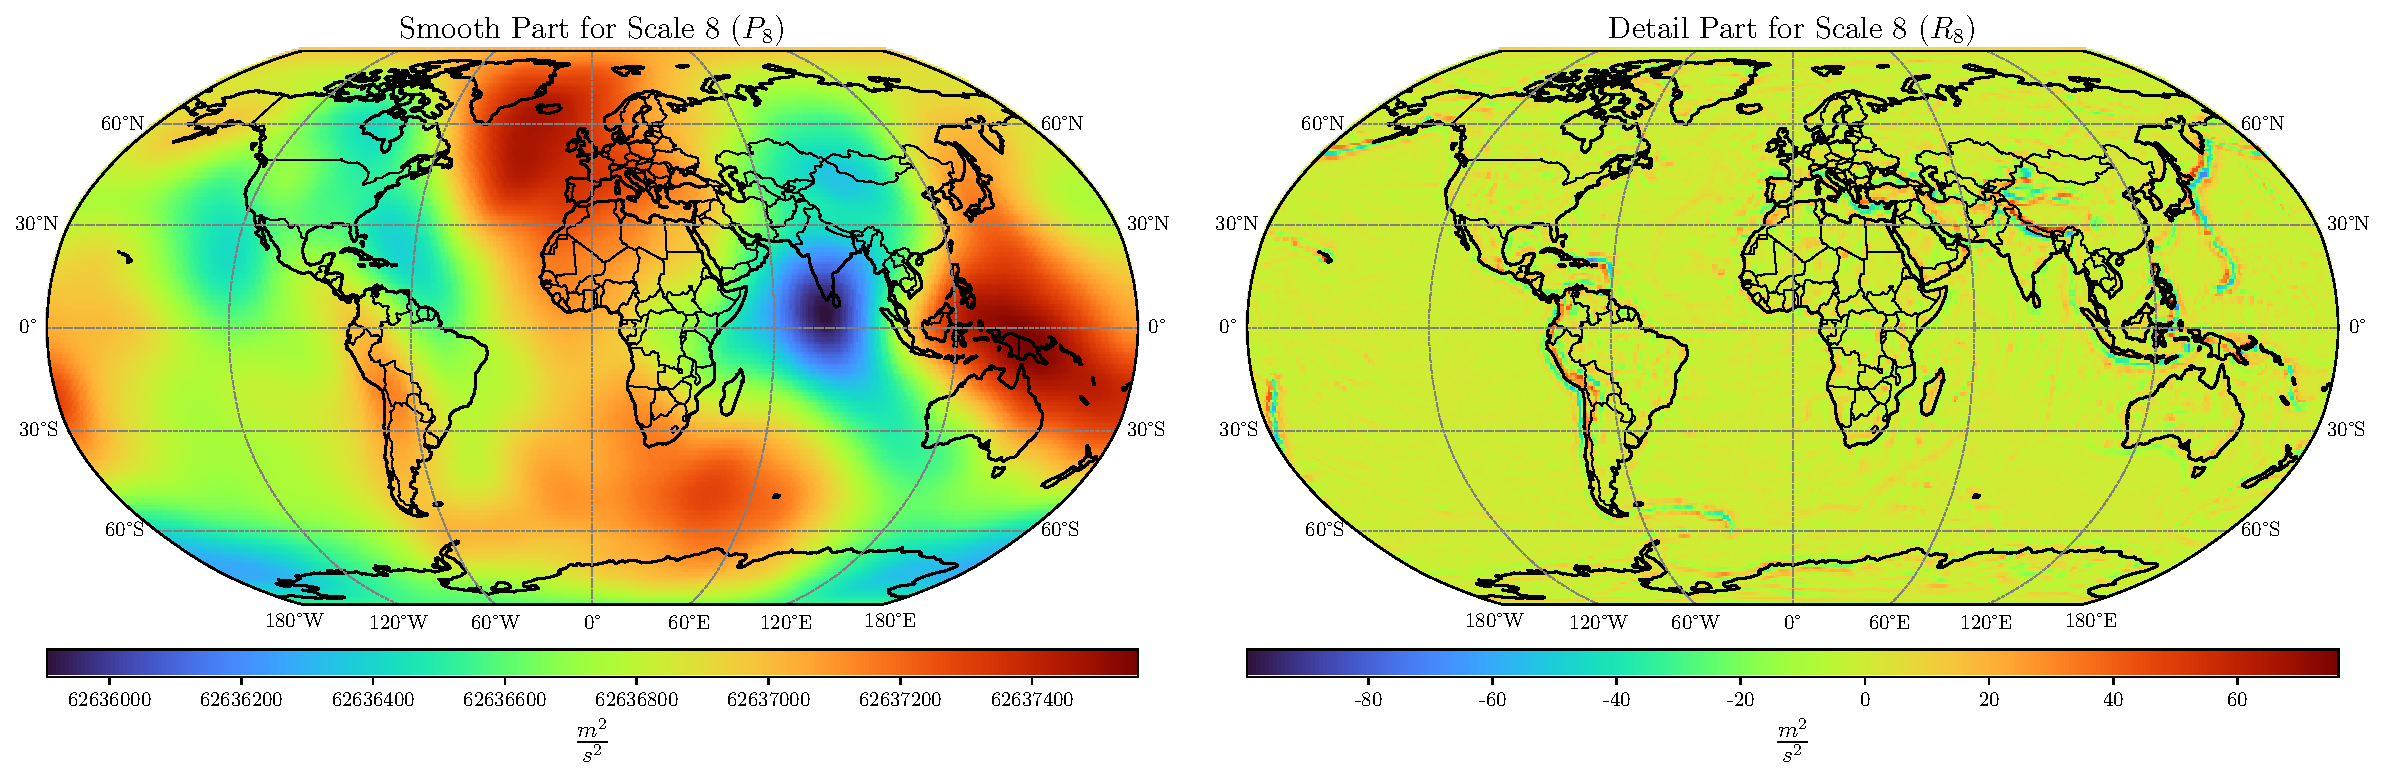
\includegraphics[width=16cm]{../Outputs/Plots/Outputs_Scale8.pdf}
		\caption{Smooth and detail part of scale 8.}
		\label{fig:Results8}
	\end{figure}
	
	
	
\end{document}